\section{Communication protocols} \label{cha:comprot}
There are multiple methods for communicating in a network, and such a procedure is called a protocol \cite{protocol}. A protocol is a set of rules regarding for example the information format, procedures for sending and receiving, error discovery and handling, and it can be implemented in both hardware and software.
In this section, some wireless network communication protocols are presented. 
First flooding protocols, followed by routing protocols.

There are many protocols and multiple groups of protocols, therein routing and flooding. 
Routing will transfer the information to the destination node through a determined route, whereas the flooding method will notify all nodes within reach to distribute the information forward, and this will repeat until all nodes has transmitted the information, and hence the destination node also has received the information.

%In networking, a protocol is a special set of rules and standards for how nodes(devices) would interacts with each other\cite{Protocol_difinition}.
%Well known protocols could be TCP/IP(Transmission Control Protocol/Internet Protocol), which affects every device connected to the internet.

Main node in this section is defined as the computer that handles that requests or sends the initial packet.
Packets are data sent though out the network. A packet can contain data to be delivered, or metadata to keep track of the packet, such as the sender ID of the packet.


\subsection{Flooding protocols}\label{cha:floodingSec}
Flooding in networks is a protocol used to deliver data throughout a network.
There are two kind of flooding: uncontrolled flooding and controlled flooding\cite{controlled_flooding}.

Uncontrolled flooding is the broadcasting of a packet, with a particular recipient, but without a particular route to reach the destination. Each node receiving the packet will repeat it to all of its neighbors, and they will repeat it again to theirs. This causes the packet to reach all nodes in the network, but it can cause communication loops. \cite{flooding}.

Controlled flooding is flooding protocols with filters or other measures to make it more reliable or efficient than the uncontrolled, hence avoiding cycles and broadcast \cite{controlled_flooding}.
Examples of such algorithms are Sequence Number Controlled Flooding (SNCF) and Reverse Path Flooding (RPF).
With SNCF, each node have its own address that is delivered with each data packet it transmits.
If a node receive a packet multiple times with the same unique id, the packet is discarded, so only one instance of the packet is transmitted.
In RPF, a node will forward a copy of a received packet, no matter the origin.
RPF expects that the original transmitted packet will be copied by the nodes in a path to the destination and eventual delivered\cite{RPF}.

Advantages of flooding, is that if there exists a route from the source to the destination, a packet will be delivered, and up to multiple times, depending on the implemented protocol.
Since some flooding algorithms utilizes every route in the network, it will also transfer packets through the shortest path\cite{flooding}.

Disadvantages can be that the bandwidth is wasted, since flooding is a very costly algorithm since it utilize every route.
Packets can be duplicated in the network, further increasing bandwidth load.
Duplicate packet may loop in the system forever, if no prevention is made \cite{flooding}.


\subsection{Time division multiple access}
Time division multiple access(TDMA) is an access protocol that divides a single channel into smaller time slots.
Each time slot is assigned to a single node, while every timeslot, are on the same channel.
Each timeslot is active a short period of time, allowing the assigned node to transmit, before the next node in the queue get time to transmit\cite{TDMA}.

%TDMA is, for example, used in the T1 telecommunication transmission system.\todo{relevance? what is T1?}
%Each T1 channels carry up to 24 voice telephone connections, where each connection covers 300 Hz to 3000Hz and is digitized at an 8-kHz rate, which is two times the highest frequency component needed to retain all the analog content.\todo{not protocol approach. very specific implementation example.}
\begin{figure}[!h]
	\centering
	\makebox[\textwidth][c]{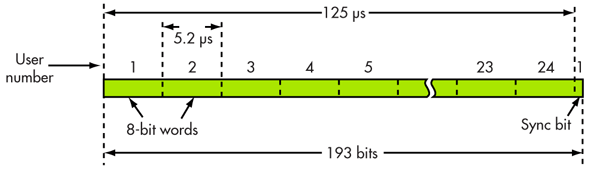
\includegraphics[width=1\textwidth]{figures/TDMA.png}}
	\caption{Illustration of the TDMA access method in the T1 protocol\cite{TDMA}.}
	\label{fig:TDMAfigure}
\end{figure}

In \figref{TDMAfigure} it is seen how the channel is split up into 24 smaller pieces. 
After the queue of timeslot there exists a bit, called the "Sync bit" as seen on the figure, that is used for synchronization.
Dividing the channel into smaller bites have little effect on the nodes transmission, because the shift between each time slot happens so fast.
This gives the illusion of each node communicating with no interruptions, even though each one is only assigned 1/24 of the total bandwidth on the channel.

TDMA can be used for any system that require several device to use the same channel, where interference can be a problem.
For example is radio transmitters a great fondness for causing interference, and that is in one of the areas TDMA can be used.\cite{interferance_protocols}



%\subsection{Radio Link Protocol}
%Radio Link protocol(RLP) is a automatic repeat request(ARQ)\footnote{An error-control method for data transmission that uses acknowledgements and timeouts} fragmentation protocol used over a wireless air interface.
%Most air interface protocols have a packet loss of up to 1\% which is intolerable when handling sensitive data.
%RLP detects losses in packets and with a retransmission tries to bring down the losses.
%The retransmission can bring the loss down to 0.1\% to 0.0001\%.
%This loss rate is more tolerable when handling sensitive and precise data.

%RPL cannot request a certain payload size from the air interface, the air interface scheduler instead determines the packet size, based on changing channel conditions constantly.
%Most of the other fragmentation protocols, such as 802.11b\footnote{An wireless networking specification} and IP, determine a payload of a certain size by the upper layers, and call upon the MAC.
%These protocols are not as flexible as RLP, and sometime fail transition during small fades in a wireless environment.\cite{MobileComm}

%RLP is used to make a more fail-safe environment for the transmitted data, and to ensure nothing is lost on the way.
%The Radio Link Protocol is typically used in cellular transmission.

\subsection{Dynamic Source Routing protocol}
The Dynamic Source Routing protocol (DSR) is a simple routing protocol designed specifically for use in wireless ad-hoc networks.
With DSR, the network is completely self-organizing and self-configuring, requiring no administration or existing network structure \cite{DSR}. 
As nodes can be added and removed as desired, the protocol automatically determine and maintain the routing of the packets through the network.
Since the number or sequence of nodes in a network, may change at any time, the topology may be quite rapidly changing.
DSR works on demand, allowing the routing of DSR to scales automatically affecting only nodes that is needed.
The protocol provides a highly responsive service to ensure successful delivery of data packets where node may be moving around, or other changes in the network occur\cite{DSR}. 

The DSR protocol is composed of two main mechanisms that allow the discovery and maintenance of the routes in the network.

- Route discovery is the mechanism by which a node S wishing to send a packet to a destination node D, obtains a route to D.
Route Discovery is used only when S attempts to send a packet to D and does not already know a route to D.

- Route maintenance is the mechanism by which node S is able to detect, while using a route to D, if the network topology has changed such that it can no longer use its route to D, which is known as a broken route.
When Route Maintenance indicates a route is broken, S can attempt to use any other route it happens to know to D, or it can invoke Route Discovery again to find a new route for subsequent packets to D.
Route Maintenance for this route is used only when S is actually sending packets to D.

DSR is a routing protocol where packets carries a header, an ordered list of nodes which is the route.
This explicit use of routing allows the sender to select and control the route for the packets it sends.
Routing allow for load balancing, since the sender can create different routes out though the network, avoiding high throughput through few nodes.
It is also a guarantee that the routes used are loop-free, since a generated route never use the same node twice.
By including this route in the header of each packet, other nodes forwarding or overhearing any of these packets can use this information for future use\cite{DSR}.
When a node overhear a packet with a route, the route is stored locally on the node.
The node can then use the route to forward messages, if its old route is unavailable.

\subsection{Ad-hoc On-Demand Distance Vector Routing}\label{cha:AOVD1}
Ad-hoc On-Demand Distance Vector(AODV) routing algorithm is a routing protocol designed for ad-hoc networks. 
It is an on-demand algorithm, meaning that it builds routes between nodes only as necessary by main nodes \cite{AOVD1}.

AODV is a network where only the nodes within reach of a newly added node is affected by the addition.
The transmission route in AODV is managed so that only nodes in the direct route are active.
The protocol can determine multiple routes between a main node and a destination, but only a single one is implemented, the route is not necessarily the shortest \cite{AOVD1}.

A disadvantage to AODV is that if a single route breaks, for example due to a defect node, it is not possible to know whether other routes exists.
A new route discovery in AODV is to be carried out before knowing if there exist a route.
If a link between nodes is broken, and it does not affect an ongoing transmission, no notification back to the main node occurs.

When a node is to forward a packet to a specified destination, it checks its routing table to determine if there currently exists a route to the destination.
The routing table is a table over every route though the node to any other, already discovered, destination.
If there already exist a route, the packet will be delivered to the next node in the route, repeating until it arrives at the correct location.
If there does not exist a route, the node will initiate a route discovery process \cite{AOVD1}.

A route discovery process in AODV begins with the main node creating a Route Request (RREQ) packet.
The packet contains the main node's unique ID and the destination node's unique ID.
The packet is then transmitted from the main node to it's neighbours.
The unique ID of each node is then appended to the packet, to ensure the same node is not transmitting more than once.
The destination ID is to ensure the nodes in the route knows when the destination node is reached.
A simple AODV network can be seen in \figref{AODVfigure}, where S and D represent the main node and destination. It is visualized how the route discovery is invoked using the RREQ packet.\cite{AOVD2}

\begin{figure}[!h]
	\centering
	\makebox[\textwidth][c]{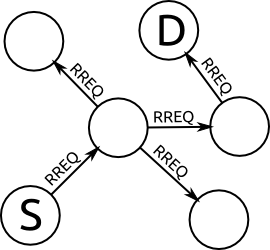
\includegraphics[width=0.4\textwidth]{figures/AODV.png}}
	\caption{Illustration of the AODV route discovery.}
	\label{fig:AODVfigure}
\end{figure}

\subsection{Better Approach To Mobile Ad-hoc Networking}
Better approach to mobile ad-hoc networking (B.A.T.M.A.N) is a routing protocol for ad-hoc mesh networks, based on AODV. 
B.A.T.M.A.N is said to solve some of the more typical problems with the classical routing protocols.
Some of the problems are, some networks are unstructured, can be based on an inherently unreliable medium and dynamically change their topology\cite{BATMAN}.

When using the B.A.T.M.A.N algorithm, the approach is to share the knowledge about the most reasonable path between nodes in a network to all of the participating nodes.
Each node in the network only account for the best path to all other nodes in the system.
This results in the need for a global knowledge about local topology changes becomes unnecessary.
In addition, B.A.T.M.A.N has an event-based, but timeless, flooding mechanism that prevents the occurrence of loops in the network.

Each node in the network transmits a broadcast message(called OGMs or originator messages in B.A.T.M.A.N) to inform every node within range about its existence.
The nodes within range, then re-broadcast the OGMs, to nodes within their range, about the existence of the original initiator of this message and so on.
This can result in the network being flooded with OGMs.
OGMs are small, the typical raw packet size is 52 byte including IP and UDP overhead\cite{BATMAN}.
OGMs contain at least the address of the originator, the address of the node transmitting the packet, and a sequence number.

OGMs that follow a path where the quality of wireless connection is poor will suffer from packet loss or delay on their way through the network.
Therefore OGMs that travel on good routes will propagate faster and be more reliable\cite{BATMAN}.

In order to tell if a OGM has been received once or more than once it contains a sequence number, given by the originator of the OGM.
Each node re-broadcasts each received OGM at most once and only those received from the neighbour which has been identified as the currently best next hop (best ranking neighbour) towards the original initiator of the OGM.

This way the OGMs are flooded selectively through the network and inform the receiving nodes about other node's existence. 
A node X will learn about the existence of a node Y in the distance by receiving it's OGMs, when OGMs of node Y are rebroadcasted by its neighbours.

The algorithm then selects this neighbour as the currently best next hop to the originator of the message and configures its routing table respectively \cite{BATMAN}.

\subsection{Protocol comparison}
Below is a comparison table with the protocol discuses in this chapter.
The four different protocols is compared in what route metric they are using, if they are loop free, support of load balancing, how reliable they are, and the estimated throughput.
This table is to create an overview of the protocols and to support a later choice of protocol of implementation.

\todo{actually compare the protocols?}

\begin{table}[!ht]
\caption{Protocol comparison.}
\label{my-label}
\makebox[\linewidth]{
\begin{tabular}{|l|c|c|c|c|c|c|}
\hline
            & Ad hoc & Route metrics                                                                     & \begin{tabular}[c]{@{}c@{}}Loop \\ Free\end{tabular} & \begin{tabular}[c]{@{}c@{}}Load \\ balancing\end{tabular} & Reliability & Throughput                                                                    \\ \hline%cline{1-1}
\rowcolor[HTML]{EFEFEF} 
TDMA\cite{TDMATable}        & Yes    & \begin{tabular}[c]{@{}c@{}}Routes ensuring\\  guaranteed bandwidth\end{tabular} & Yes                                                  & Yes                                                       & High        & \begin{tabular}[c]{@{}c@{}}Decreases as more \\ nodes are added\end{tabular} \\
DSR\cite{ProtocolTable}\cite{DSR}         & Yes    & Source routing                                                                   & Yes                                                  & No                                                        & High        & \begin{tabular}[c]{@{}c@{}}Decreases as more\\  nodes are added\end{tabular} \\
\rowcolor[HTML]{EFEFEF} 
AOVD\cite{ProtocolTable}        & Yes    & \begin{tabular}[c]{@{}c@{}}Fastest \&\\ shortest path\end{tabular}               & Yes                                                  & No                                                        & High        & \begin{tabular}[c]{@{}c@{}}Poor for more\\  than 20 nodes\end{tabular}       \\
B.A.T.M.A.N\cite{BATMAN} & Yes    & \begin{tabular}[c]{@{}c@{}}Fastest \&\\ shortest path\end{tabular}               & Yes                                                  & No                                                        & High        & \begin{tabular}[c]{@{}c@{}}Good - scales\\ well with more nodes\end{tabular} \\ \hline
\end{tabular}}
\end{table}

\iffalse %temporary removed
\subsection{Flooding as a routing algorithm}\label{cha:floodingSec}
Flooding in networks, is a routing algorithm used to deliver data out though a system.
There exists two kind of flooding, uncontrolled flooding and controlled flooding.
Uncontrolled flooding is a kind of "brute force", where every node, in a network, keeps sending the same packets indefinitely out to all its neighbours within range, creating what is known as a broadcast storm.
The packet will eventually the packet will reach its destination, without knowing when\cite{flooding}.

Controlled flooding is modified algorithms to make it reliable, some of algorithms are knows as Sequence Number Controlled Flooding(SNCF) and Reverse Path Flooding(RPF).
With SNCF each node have its own address that is delivered with each data packet it transmits.
If a node receive a packet twice or more with the same address, the packet is discarded, so only one instants of the packet is working its way though the network.
In RPF, the node will forward a copy of a received packet, no matter the origin.
RPF except that the original transmitted packet will be copied by the right nodes and eventually end at the destination\cite{RPF}.

Advantaged of flooding, is that if there exists a route from the main node to the destination, a packet will be delivered, and possible multiple times.
Since some flooding algorithms utilized every route in the network, it will also transfer packets though the shortest path\cite{flooding}.

Disadvantages can be that the bandwidth is wasted, since flooding is a very costly algorithm since it utilize every route.
Packets can be duplicated in the network, future increasing bandwidth load.
Duplicate packet may loop in the system forever, if no prevention is made\cite{flooding}.

\todo{flooding: take 2}
\fi
